\begin{figure}[!t]
  \setlength{\abovecaptionskip}{4pt}
  \centering
  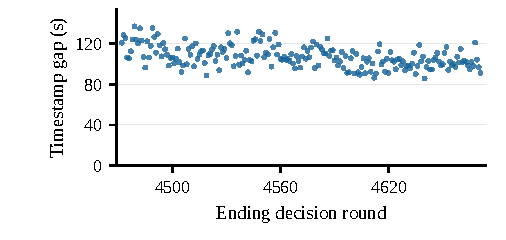
\includegraphics[width=\linewidth]{figures/fig_decision_cadence.pdf}
  \caption{\textbf{Recent adapter decisions arrive at varying intervals.}
  All 200 timestamp gaps between the latest 201 complete journal records,
  rounds 4471--4671, captured at 23:57 UTC on 3 November 2026.
  Each point subtracts the previous recorded timestamp from the current one
  and is keyed to the ending decision round. Both endpoint source lines
  and hashes are retained. These intervals include work, qualification waits
  and recording gaps; they measure record cadence, not compute time,
  single-proposal latency or learning. Scope: \cref{sec:method-status}.}
  \label{fig:decision-cadence}
\end{figure}
\FlushFloatsInPlace% keep the final cadence figure ahead of its subsection and References

\subsection{A recent decision-cadence snapshot}\label{app:decision-cadence}

\Cref{fig:decision-cadence} complements the separate utility-margin
snapshot in \cref{fig:candidate-margin-window}; the two windows do not
support a joint quality--cost comparison.
